

\section{The \sys{} confinement system}
\label{sec:system}

In this section we describe the \sys{} system.
%
Unlike existing browser security mechanisms, \sys{} provides
\emph{confinement:} it gives code access to sensitive
data while ensuring that the code cannot release that sensitive
data arbitrarily~\cite{SaltzerS75}.
%
Our confinement mechanism allows developers to enforce both policies
that are stricter than the SOP and policies that are more flexible
than the SOP (yet still safe), without imposing the limitations of CSP
and CORS.
%
Below, we first describe how one encodes policies in \sys{}, and then
the system design itself.

\subsection{Policies and confinement in \sys{}}
\label{sec:system:policy}

\begin{figure}
{\small{
\begin{webidl}
Label {
  Label Label([String])
  Label and(String or Label)
  Label or(String or Label)
  bool subsumes(Label [,Privilege])
}
\end{webidl}
\begin{webidl}
Privilege {
  Privilege FreshPrivilege()
  Privilege combine(Privilege)
  Label asLabel(Privilege)
}
\end{webidl}
}}
\vspace{-10pt}
\caption{\label{fig:APIspec} API for policy specification}
\vspace{-10pt}
\end{figure}


Conceptually, \sys{} associates a security policy with every piece of
data in the system, specifying which origins can read and write the
data.
%
Such policies are known as \emph{labels}.
%
The particular labels used by \sys{} are the \emph{DC
labels} presented in~\cite{stefan:2011:dclabels}.
%
We chose DC labels, much like Hails~\cite{giffin:2012:hails} and
Breeze~\cite{Breeze13}, because they have a simple and clear semantics, yet are
as expressive as the labels used by other practical confinement
systems~\cite{GenLabels}. Figure \ref{fig:APIspec} shows the \sys{}'s API (in a
WebIDL-like syntax) to specify policies (privileges to be
explained below).


A privacy label (henceforth just label) is a boolean formula over
origins, specifying who can read the data.\footnote{
  We note that our system also handles integrity, or trust, which
  serves as the dual of privacy.
  %
  For simplicity of exposition we omit integrity from our discussion
  and simply note that it serves as the dual of secrecy.

}
%
For example, the label
\js|Label("https://bank.ch").and("https://amazon.com")| specifies that
the data may contain sensitive information from both origins.
%
Such a label may be used by an application that compares bank
statements with Amazon purchases.
%
Importantly, the label specifies that the data should not be
propagated to a less sensitive entity, e.g., an \https{amazon.com};
\sys{} prevents the dissemination of such data to \https{amazon.com}
(either, in-browser or with XHR), since it may leak bank information.
%
Of course, if the bank wishes to share and allow \https{amazon.com} to
disseminate certain information, it can label it
\js|Label("https://bank.ch").or("https://amazon.com")|;
this disjunctive label states that either origin may disseminate the
data.

When exchanging information, the actual check performed by \sys{} is
logical implication, as implemented by the \js|Label| method
\js|subsumes|.
%
Specifically, \sys{} ensures that data labeled \js|ldata| can be only sent
to an entity labeled \js|lentity| if
\js|lentity.subsumes(ldata)| is \js|true|.
%
Intuitively this states that an entity is allowed to receive data that
is at most as sensitive as its label, i.e., the entity label
always \js|subsumes| the label of the data it can receive,
preserving the latter's privacy.
%
We refer the interested reader to~\cite{stefan:2011:dclabels} for more
details.

Rather than explicitly labeling every object (a trade-off discussed in
Section~\ref{sec:discussion}), in \sys, we associate a label with
every \emph{compartment}~\cite{wagner2011compartmental}.
%
A compartment roughly corresponds to the JavaScript heap (for
simplicity, global object) of a web page, iframe, Worker~\cite{workers},
etc.; this allows us to reason about JavaScript security semantics at
a coarse-grained level: we need only impose security checks for
cross-compartment references, references to objects within the same
compartment require no security checks since they share the same
label.
%
We sometimes abuse terminology and use the phrase  ``label of a
browsing context'' to mean the label on the compartment that contains
the browsing context's document, even though, for example, Worker
compartments do not have a document or browsing
context~\cite{workers}.
 
The label of the compartment serves as a ``taint,'' indicating the
sensitivity of data contained within the compartment, i.e., the
sensitivity of the data the code executing within the browsing context
has read.
%
For example, the compartment label
\js|Label("https://bank.ch").and("https://amazon.com")| specifies that
the compartment may contain data sensitive to \https{bank.ch} and
\https{amazon.com}.
%
To preserve the privacy of this data, \sys{}, in turn, uses the
compartment label to confine code by restricting where it can write.
%
Specifically, code is restricted to communicating with browsing
contexts (e.g., via \js|postMessage|) whose labels subsume the current
label of the browsing context.
%
Similarly, performing network requests and accessing persistent storage is
dictated by the relationship of the context label and implicit labels of these
end-points.  


\sys{} introduces \emph{privileges} to make the SOP notion of
authority (of code) over page content explicit.
%
A privilege is an unforgeable object with which code can assert the
authority of the corresponding origin (e.g., to declassify that
origin's data).
%
In \sys, a browsing context is given the privilege corresponding to
the page origin.
%
In turn, the privilege is used when performing any \js|subsumes|
label checks.
%
For example, a script running in an \https{amazon.com} page has the
privilege corresponding to the \https{amazon.com} origin.
%
Without this privilege the script cannot perform any XHR requests
if the context label is
\js|Label("https://bank.ch").and("https://amazon.com")|:
the label of an end-point cannot subsume such a conjunctive policy.
%
However, with the  \https{amazon.com} privilege, the code can perform
XHR requests to \https{bank.ch}, and in doing so, it is effectively
declassifying any \https{amazon.com}-sensitive data used in the
request.
 
Importantly, code cannot synthesize arbitrary privileges.
%
For example a script executing in a \https{amazon.com} browsing
context cannot create a privilege for \https{bank.ch} and declassify
arbitrary bank data---this would trivially violate any confinement
guarantees.
%
In our system, code can only create the empty privilege (which is
simply the JavaScript \js|null| object) and privileges corresponding
to fresh, unique origins (created with the \js|FreshPrivilege|
constructor).
%
As in HiStar~\cite{Zeldovich:2006}, the ability to generate fresh privileges
ensures that all browsing contexts are egalitarian, i.e., a child iframe is no
less trustworthy than its containing parent.  Figure~\ref{systemAPI} shows the
API to handle privileges (primitives \js|combine| and \js|asLabel| to be 
explained in the next subsection). 


In an ideal confinement system, code can read arbitrary data at the
cost of raising the context label and thus giving up write privileges.
%
Unfortunately, practical systems typically have covert channels which
may be exploited to leak sensitive data.
%
Hence, as in HiStar~\cite{Zeldovich:2006}, Hails~\cite{giffin:2012:hails}, and
Breeze~\cite{Breeze13} we associate a \emph{clearance}---which is
simply a label---with every compartment.
%
Clearance imposes a limit on the kind of data a compartment can have,
i.e., it is an upper-bound on compartment label, and thus the kind of
data a piece of code executing in the compartment can access.

For completeness, we summarize  \sys{}'s API for compartments
in Figure~\ref{systemAPI}. In the next subsection, 
we explain the purpose of the different primitives through examples. 
We remark that \sys{}'s API is designed to be minimalistic, and as such, it only
consists on the primitives shown in Figures~\ref{fig:APIspec} and
\ref{systemAPI}.

In the rest of this section, we expand on the \sys{} design by
introducing mechanisms that meet the requirements of the four
example applications described in Section~\ref{sec:goals}.
%% through
%% three concrete examples: 
%% a password-strength checker (Section~\ref{sec:system:worker}),
%% a password manager (Section~\ref{sec:system:iframe}), 
%% a third-party mashup (Section~\ref{sec:system:mashup}), and
%% a library that converts phone numbers to links
%% (Section~\ref{sec:system:script}--Section~\ref{sec:system:extension}).
%
%For completeness, we summarize the different system components,
%security mechanisms, and DOM API (using WebIDL-like syntax), in
%Table~\toref{table:components}.


\begin{figure}
{\small
\begin{webidl}
SWAPI {
  attribute Label label
  attribute Label clearance 
  attribute Privilege privilege
}
\end{webidl}
\begin{webidl}
LWorker {
  LWorker LWorker(String, Label
                  [, Privilege, Window])
  LWorker SOLWorker(String, Label)
  postMessage(Object [,Label])
  attribute EventHandler onmessage
}
\end{webidl}
}
\vspace{-10pt}
\caption{\label{systemAPI} API for compartments}
\vspace{-10pt}
\end{figure}


\subsection{Confining third-party DOM-less code}
\label{sec:system:worker}

%\para{\sys{} approach}
%
%
%% (Rather today's mechanisms give developers a limited form of access
%% control.)
%
\sys{} allows developers to treat a piece of code as untrusted and
confine it. This functionality is instrumental in supporting the
password-checker application, which we use as a running example.
%
We first consider the confinement of ``DOM-less'' code; in
Sections~\ref{sec:system:iframe} and \ref{sec:system:extension} we
address confinement of third-party code with access to the DOM.

As noted in Section~\ref{sec:goals}, and previously observed
in~\cite{Ingram:2012}, workers are a good first step towards reasoning
about the security implications of untrusted code that does not need
to access the DOM, since they provide a clean, isolated environment
within which untrusted code can be executed.
%
Hence, we extend the Worker DOM API~\cite{workers} with a
Labeled-Worker (LWorker).
%
Like a standard worker, an LWorker executes a piece of code in a fresh
compartment that exposes a limited set of objects and properties.
%
Concretely, we expose the \sys{} API (including the \js|LWorker|
constructor used to construct additional labeled Workers), the \xhr{}
constructor used to perform network requests, and
\js|onmessage|/\js|postMessage|used for communicating with the
parent.
%
Different from the \js|Worker| constructor, the \js|LWorker|
constructor takes three additional arguments: a label that specifies the
clearance on the code running in the worker, an optional privilege
to grant the worker, and an optional window object to attach to the worker.
%
We discuss the role of the latter two arguments in Sections~\ref{sec:system:script}--\ref{sec:system:extension}.

For example, we create a new LWorker that executes the
password-strength checker code as follows:
\begin{jscode}
var url = "https://checker.biz/checker.js";
var label = new Label(location.origin);
// 1. Execute checker in new worker
var checker = new LWorker(url, label);
\end{jscode}
%
Assuming the browsing context (main page) creating the worker has not
enabled \emph{confinement-mode}, \sys{} first enables confinement-mode
and sets the browsing context label to the public label \js|Label()|.
%
In general, a script can explicitly enable confinement-mode or set
the compartment label to a label more restricting than the current
label; when enabling confinement-mode, \sys{} takes a
permissive approach and sets the initial browsing context label to the
public label.
 
Subsequently, \sys{} ensures that the page is allowed to make
a request to \js|url| to fetch the source code.
%
As with loading content (e.g., images, styles and scripts), writing to
storage (e.g., cookies), or performing explicit network requests with
\xhr{}, \sys{} asserts that, given the current context privileges, the
label of the resource---which is implicitly \js|Label(|\emph{resource
origin}\js|)|---subsumes the browsing context label.
%
In this case, the resource label \js|Label("https://checker.biz")|
subsumes the context label \js|Label()| and thus fetching the script
is permitted.

Before executing the fetched script in the new worker compartment, \sys{}
ensures that the label of the worker is at least as restricting as the
current label.
%
This check ensures that the page cannot declassify data by laundering
it through a worker whose label is less sensitive than the context
label.
%
\iffigures
\ifcompletefigures
As shown in Figure~\toref{fig:strength-1}, 
\fi
\fi
\sys{} then starts
executing the checker code in the LWorker; the initial label of the
worker compartment is set to that of the parent (in this case, the
public label).
%
Our use of labeled workers in this fashion is similar to the executing code in
LIO's \js|toLabeled| block~\cite{stefan:2011:flexible} and Breeze's
\js|bracket|~\cite{Breeze13}.
 
At this point, the code executing in the labeled worker can fetch
data, such as a list of weak passwords from any origin,
CORS-permitting.
%
It is important to note that since the password-strength checker has
not yet read any sensitive data, which is reflected in the compartment
label, this is a safe operation, i.e., making the request does not
leak any information.
%
Only once the code decides to inspect the password should it no
longer be able to perform such arbitrary network requests.

To retrieve the password, the password-strength checker registers a
message-event handler, which is invoked when the parent sends it a
message whose label is subsumed by the checker's label (step 3, on the
right):
\begin{jscode}
// checker.js ...
// SWAPI.label == Label()
function computeStrength(pass) { /* ... */ }

// 2. Raise context label & register handler
SWAPI.label = SWAPI.clearance;
// SWAPI.label == Label("https://instagra.me")
onmessage = function(event) {
  var password = event.data;
  // 4. Check score & send it to parent:
  postMessage(computeStrength(password));
};
\end{jscode}
%
Importantly, the worker first raises the context label to the
clearance---which is the worker label---by setting \js|SWAPI.label|.
%
In doing so, the code is effectively stating that it is ready to
receive data at sensitivity level \https{instagra.me}, at the cost of
giving up arbitrary communication privileges.
%
\iffigures
\ifcompletefigures
As shown in Figure~\toref{fig:strength-3}, the 
\else
The
\fi
\fi
checker can now receive
sensitive data (the password), but, for example, can only use \xhr{} to
communicate with \https{instagra.me};
%
performing arbitrary network requests or creating arbitrarily-labeled
workers is no longer permitted.

Next, the page sends the LWorker the
password via \js|postMessage|, and registers a message handler to
receive the strength score:
\begin{jscode}
var password = 
 document.getElementById("password").value;
// 3. Send checker password 
checker.postMessage(password, l);
// 5. Get score
checker.onmessage = function(event) {
  var score = event.data; 
  // ...
}
\end{jscode}
Here, \js|postMessage| additionally takes the label of the message
\js|l|, which must be subsumed by both the browsing context clearance
and worker label.
%
(If an explicit label is not supplied, \sys{} uses the browsing
context label as the message label.)
%
We use this label to ensure that the receiver's message handler is
dispatched only if its browsing context label is at least as sensitive
as \js|l|---thus preserving the privacy of the password.

In the final step, the event handler, which is called with the
parent-supplied password, invokes the underlying password-strength
checking function \js|computeStrength|.
%
The result of this function is returned to the page via
\js|postMessage|.
%
The event handler registered by the page 
\iffigures
\ifcompletefigures
(step 5), as shown in Figure~\toref{fig:system:strength-4}, 
\else
(step 5)
\fi
\fi
is dispatched if the label of
the page subsumes the message label (which is the worker's compartment
label).

\iffigures
\ifcompletefigures
We show the full life-cycle of this application in
Figure~\toref{fig:system:strength}.
\fi
\fi
%
In this example, we relied on the page having ownership of the
\https{instagra.me} privilege as to avoid tainting the browsing
context when reading the score from the worker.
%
Unfortunately, this also means that our confinement of the checker
code is limited: we cannot label the worker with this label and
restrict it from using XHR to self-exfiltrate data to
\https{instagra.me}.
%
Instead, the page must label the worker with a unique origin that does
not correspond to an actual host, as to prevent it from leaking data
using XHR, yet still has the privilege to communicate with its parent.

This is precisely the role of fresh privileges.
%
A fresh privilege corresponds to a unique origin whose scheme is
prefixed by \texttt{x-swapi}; the fake protocol ensures that the
\xhr{} constructor cannot be used to make requests.
%
Hence, to fully confine the password-strength checker we modify the
\https{instagra.me} page to first create a fresh privilege and use the
corresponding label when creating the LWorker.
%
Th modified code is shown below.
\begin{jscode}
// Create fresh unique privilege
var p = new FreshPrivilege();
// Take ownership of this privilege
SWAPI.privilege = p.combine(SWAPI.privilege);
// Use it to confine the worker completely:
var checker = new LWorker(url, p.asLabel);
// As before ..
var password = 
 document.getElementById("password").value;
// 3. Send checker password 
checker.postMessage(password, p.asLabel);
// ...
\end{jscode}

We remarks that, different from current approaches, our system
provides a client-side approach to flexibly and fully confining
untrusted code:
%
the strength checker can perform arbitrary XHR until it raises its
label to register the \js|onmessage| handler that will inspect the
sensitive password; from this point on it can only communicate with
the parent.
%
This is in contrast to either giving the checker irrevocable network
access or none at all.
%
Importantly, our first-class workers and privileges makes security a
first class citizen: not only can the page consider the checker
untrusted, but the checker can itself create fresh privileges and 
LWorkers in which it can execute code it itself does not consider
trustworthy!

\subsection{Cross-iframe confinement}
\label{sec:system:iframe}
%Password manager 

In the password strength-checker application, the \https{instagra.me}
page effectively imposed the requirement that the password-strength
checker discard its network communication capabilities by raising the
compartment label sufficiently high, before reading the (labeled)
password.
%
More generally, by associating a label with every browsing context and
restricting read- and write-effects according to it, \sys{}'s
confinement mechanism can give developers a means for controlling
where users' data can flow, even after the data is made available to
untrusted browsing contexts. \sys{} thus meets the requirement of
confining untrusted code that computes with sensitive data.

%\para{\sys{} approach}
%
With \sys{}, we can leverage confinement to build a password manager
web application that does not force the user to place complete trust on 
any of the participating parties. We use the password manager as a
running example of this use of confinement.
%
Our password manager is divided into two mutually distrusting
components: a management layer (provided by e.g., \https{pwd.eff.org})
that interacts with the user, 
%to store and fetch credentials, 
and a storage layer (provided by e.g., \https{dropcu.be}) that provides a
simple
%---in effect, labeled---
%A bit confusing describing it at this point
server-side storage API for the
management layer.
%
The mutual distrust between the layers is instrumental---yet, without
confinement not sufficient---to ensuring that neither party can
individually compromise the user's privacy (and would thus have to be
trusted in full).
%

%
Though a user can use such a password manager to store and fetch secrets
directly, for simplicity, we assume that a website (e.g., \https{fb.com})
integrates with the manager in order to save and retrieve login
credentials,\footnote{ In Section~\ref{sec:implementation} we describe an
  untrusted extension system that can be used to inject the password-manager
  specific code into the integrator page.  }
\iffigures
\begin{figure}
\begin{center}
% I printed out, and it reads well!
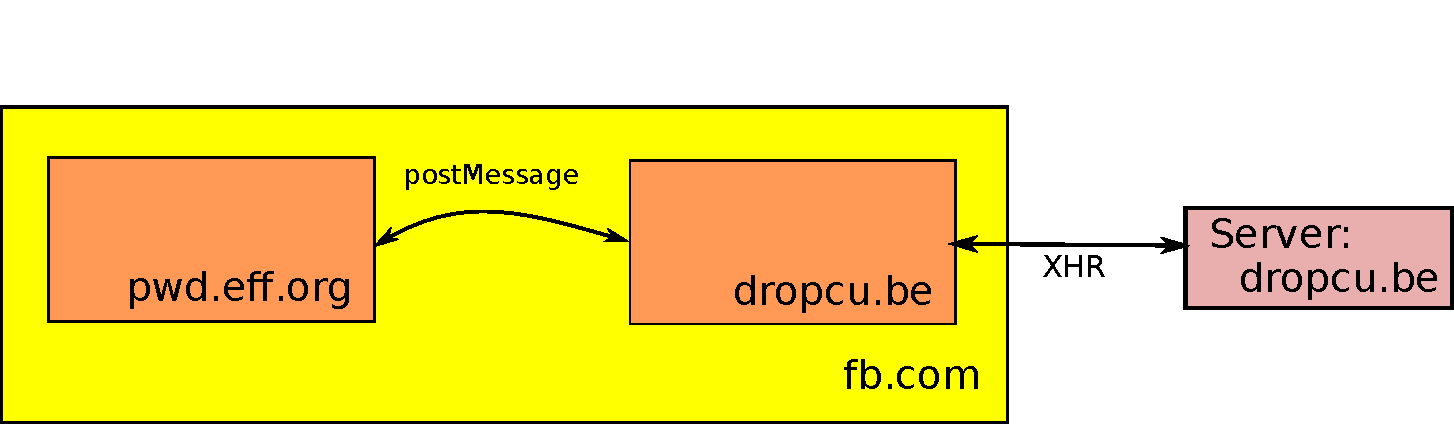
\includegraphics[scale=0.35]{pmanager.pdf}
\end{center}
\vspace{-10pt}
\caption{\label{fig:manager-s-1} Password manager architecture}
\vspace{-10pt}
\end{figure}
 as shown in
Figure~\toref{fig:manager-s-1}.
\else
.
\fi
%
Without loss of generality, we also assume that encryption and
decryption is carried out on the client-side by the management layer.
%
In this architecture, the security guarantees and trust concerns
are as follows:
\begin{enumerate}[i)]
\item The management layer never learns the site-specific (\https{fb.com})
  credentials. The user only needs to trust this component with their master
  password. Importantly, without the collusion of the storage layer, the
  management layer cannot exploit the master password in order to reveal
  credentials.

  %
  To eliminate this trust, users can inspect the management layer's
  browsing context label, either using standard developer tools or by
  right-clicking on the page (a functionality implemented by our
  supporting extension, describe in Section~\ref{sec:implementation}),
  and only supply the master password if the label ensures that the
  page cannot disseminate the password arbitrarily.
  %

\item The storage layer never learns the site-specific credentials or
  master password. The user only needs to trust this layer to not
  collude with the management layer (and vice-versa). This is a
  realistic assumption given a decentralized environment like the web.

\item Finally, the integrator never learns the master password or
  credentials private to other websites (e.g., \https{goo.gl}).
\end{enumerate}
%
It is important that the above guarantees be preserved when the
password manager is used to both save and retrieve credentials.
%
Below, we respectively describe the interaction of all the components
in saving and retrieving credentials.

\subpara{Saving credentials}
%
To save credentials, the integrator, \https{fb.com}, first creates two
iframes: one containing the \https{pwd.eff.org} management layer and
another containing the \https{dropcu.be} storage layer.
%
As part of the initialization process, the management layer saves a
pointer to the storage layer (via \js|window.parent.frames|), both
layers register \js|onmessage| event handlers, and the expected
sensitivity of data, i.e., labels, to be exchanged is shared.
%
Next, the integrator sends the credentials to the management
layer via \js|postMessage|.
%
The label of the message is
\js|Label("https://fb.com").or("https://dropcu.be")|; this label
ensures that the management layer can only receive the message if it
has raised its context label so that it subsumes the label of the
message, which subsequently limits it to communicating with the
\https{fb.com} and \https{dropcu.be} layers.\footnote{
  To confine the management layer more strictly, the message can be
  labeled with a label corresponding to a fresh origin generated by
  \https{fb.com}, the privilege to which is granted to the storage
  layer. 
}

In general, and as in the LWorker case, the browsing context's
\js|onmessage| handler is only dispatched if the context label
subsumes the message label.
%
This restriction ensures that the browsing context label is
sufficiently strict to protect the privacy of the message.
%
For content (as opposed to workers), the restriction does not solely
amount to limiting the usage of \js|postMessage| and the \xhr{}
constructor.
%
Rather, \sys{} restricts all network, storage and
cross-browsing-context communication.
%
Specifically, just as sending a \js|postMessage| requires the context
label be subsumed by the message label, when loading content (e.g.,
with \js|<img>|, \js|<script>|, etc.), writing to local storage (e.g.,
with \js|document.cookie|), performing explicit HTTP requests (with
\xhr{}), or navigating the browsing context, we require that the
context label be subsumed by the (implicit) label of the resource.
%
This ensures that the action (which is effectively a write) does not
leak any information from the context to a less-sensitive entity.
%
(Of course, in all label comparisons, the context privileges are taken
into consideration.)
%
 
Returning to our password manager, upon receiving the credentials
(\js|credentials|) via the \js|onmessage| handler, the management
layer requests the master password (\js|mpass|) from the user, 
generates a salt (\js|salt|), and encryption key $k =
H(\texttt{mpass}\|\texttt{"}\https{fb.com}\texttt{"}\|\texttt{salt})$
\iffigures
\ifcompletefigures
,as shown in Figure~\toref{fig:manager-s-2}
\fi
\fi
.
%
Here, $H$ is a hash function such as SHA-256.
%
We use the integrator origin, in addition to the master password and
salt, to ensure that a malicious storage layer will not be able to
confuse the management layer, during the retrieval process, into
decrypting \https{fb.com}'s credentials when invoked by a different
integrator, e.g., \https{goo.gl}.

% 
After the key generation, the management layer encrypts the
credentials using function \js|E| (e.g., AES), and sends
\js|E|$_k$\js|(credentials)| and the \js|salt| via \js|postMessage| to
the storage layer.
%
Assuming that the label of the message subsumes
\js|Label("https://dropcu.be")|, the storage layer's \js|onmessage|
handler will be dispatched. 
%
Since the storage layer frame has the \https{dropcu.be} privilege, it
does not need to raise its compartment label; this fact allows the
storage layer to use XHR to send the data to the \https{dropcu.be}
server.
 
We note that, in addition to the credentials and salt, the storage
layer also stores the origin of the parent, i.e., \https{fb.com}, as
meta-data (label) identifying for whom the data is being stored.
%
Rather than having the management layer provide this meta-data to the
storage layer alongside the encrypted credentials, by having
\https{fb.com} create the frame in the initialization stage, we ensure
that a malicious management layer cannot confuse the storage layer
into associating \https{fb.com}'s encrypted data with a different
origin, e.g., \https{goo.gl}, thus allowing it to be leaked during
the retrieval process.

\subpara{Retrieving credentials}
%
As in the case of saving credentials, the integrator, \https{fb.com},
creates two frames containing the management and storage layers.
%
In this scenario, the storage layer retrieves the encrypted credentials
\js|E|$_k$\js|(credentials)|, salt and ownership meta-data (in this
case, \https{fb.com}) and registers an \js|onmessage| event handler,
that responds to the management layer's ``fetch'' request.
A simplified handler is shown below.
\begin{jscode}
function handler(event) {
  // ... check origin ...
  // owner == "https://fb.com"
  // credentials == E_k(...)
  var l = new Label(owner);
  event.origin.postMessage(credentials, l);
} 
window.addEventListener("message", handler);
\end{jscode}
This handler simply replies via \js|postMessage| with the credentials.
%
Importantly, however, the message is labeled with the origin meta-data
retrieved from the server.
%
This ensures that the browsing context label of the frame requesting
the credentials---the management layer---must subsume the label of the
message. 
%
This restriction guarantees that, even if the management layer did not encrypt the
credentials during the save procedure, it cannot learn and
exfiltrate the credentials through the retrieval process; this
label ensures that it can only disseminate the credentials to the
corresponding owner (\https{fb.com}, in this case).
%

Like the storage layer, in this scenario, the management layer first
registers a message handler to receive the encrypted credentials, and
via \js|window.parent.frames|, it retrieves a pointer to the storage
layer.
%
\iffigures
\ifcompletefigures
As shown in Figure~\toref{fig:manager-r-2}, after 
\fi
\else
After
\fi
raising the
compartment label to \js|Label("https://fb.com")|, the management
layer sends the storage a ``fetch'' message, requesting the encrypted
credentials.
%
%
Subsequently, the storage layer's handler (defined above) is triggered
and the message containing the encrypted
credentials and salt is sent to the management layer.
%
At this point, its message handler is dispatched (since the management
layer's context label subsumes the label of the storage layer message)
and the master password (\js|mpass|) is retrieved from the user. 
%
Using the master password and salt, the management layer reconstructs
the key $k$, using it to decrypt the encrypted credentials.
%
These decrypted credentials are then sent (via \js|postMessage|) to
the \https{fb.com} browsing context.
%
We note that, as imposed by the storage layer, the management layers'
context label, \js|Label("https://fb.com")|, prevents it from
disseminating the data to any other origin.
%
Finally
\iffigures
\ifcompletefigures
, as shown in Figure~\toref{fig:manager-r-3}, 
\fi
\fi
\https{fb.com},
whose label remains public carries out the login procedure, i.e., it
submit the login form.

\para{Another example: encrypted online documents}
The design pattern used for the password manager can be exploited in other
scenarios. To illustrate this point, we implemented a prototype of a
mashup capable of handling encrypted on-line documents.
%Companies often argue against using on-line documents services (like Google
%Docs) due to privacy issues, i.e., they do not want Google to store sensitive
%information present in such documents. Using a similar architecture as the
%password manager, we implement a prototype of a mashup capable to handle
%encrypted on-line documents. 
This prototype shows the feasibility of our approach in combining
services such as online document providers (e.g., Google Docs)
and encryption processes. In this system, once encryption keys are configured,
the encryption and decryption are performed in a mostly transparent
manner.
The goal of the mashup is to allow the user to use a document editor,
while ensuring that the editor-provider can only store encrypted data,
as enforced by an encryption ``provider.''

Concretely, our prototype creates relies on three iframes: an outermost,
labeled \js|gdocs.com|, a mediary encryption layer, labeled
\js|encrypt.com|, and an innermost one labeled \js|gdocs.com|.
The innermost frame contains the actual document editor (that cannot
communicate with anything except the parent frame), while the middle
layer seven as an encryption mediary between the editor and outer-most
frame that communicates with the \js|gdocs.com| servers.

To enforce the aforementioned security policy we use a small
bootstrapping protocol between the middle and innermost frames.
Specifically,
once the middle, encryption-layer, frame is
loaded, it starts an authentication process with the innermost,
editor, frame before any
editing is allowed. To this end, it sends a token to the innermost
frame with the label \js|Label("https://gdocs.com").and("https://encrypt.com")|.
This message requires that innermost frame be (at least) tainted with
the described label, and as a result, restricted from performing any network
requests; this ensures that the innermost editor cannot leak
the plain document as it is composed to \js|gdocs.com|. Once the
innermost frame receives this
message, it replies to the encryption layer with the token.
The encryption-layer, in turn, verifies the token, the receipt of which ensures
that the editor-layer is confined to solely communicating with its
parent. At this point, the user
can start editing the document.

When saving the document, the document is
sent (via \js|postMessage|) to the middle frame for encryption.
The encryption layer, exercises its privilege \https{encrypt.com} to
send the encrypted document, labeled \js|Label("https://gdocs.com")|,
to the outermost frame, which, in turn, uses XHR to store the
document on \js|gdocs.com| servers.


\subsection{Privilege separation within iframes}
\label{sec:system:script}

The confinement system presented thus far requires developers to
compartmentalize components/libraries of different trustworthiness into
multiple labeled iframes/workers.
%
%% Though this is sufficient for many libraries and mashups, placing a library
%% such a jQuery, which inherently traverses and modifies many parts of the DOM,
%% in a separate iframe/worker is not practical: developers use jQuery as a
%% JavaScript domain specific language with which they build application.
%
We now return to the \https{bank.ch} example application discussed in
Section~\ref{sec:goals}. How can we ensure that a library such as
jQuery does not leak the user's bank statement?

Rather than attempt to solely confine jQuery within such a page, we
can take a more conservative approach and confine all the code in the
page.
%
To this end, we raise the label of the browsing context and drop the
page privileges before importing the library:
\begin{jscode}
// Raise label:
SWAPI.label = new Label(location.origin);
// Drop privileges:
SWAPI.privilege = null;
\end{jscode}
%
This ensures that the page, independent of jQuery's behavior, can only
disseminate data to \https{bank.ch}.
%
However, this also requires the jQuery library code to be hosted on
the same origin, i.e., \https{bank.ch}.
%

To allow the page to communicate with other domains, the application
must create an iframe to a \https{bank.ch} page, which is granted the
bank privilege and thus able to communicate arbitrarily with that origin.
%
The role of this child frame is to solely implement the ``trusted''
components of the application.
%
Specifically, its sole role is carry out requests (submitted via
\js|postMessage|) for the parent, after asserting that the request is
safe (e.g., updating local storage to reflect the last page view,
etc.).


Unfortunately, adapting a web page to work with a privilege frame 
is far from trivial. There are several reasons for that. 
%such compartmentalization is not trivial for 
%realistic scenarios.
%
Firstly, the trusted iframe cannot inspect the DOM (state) of the parent frame
and make decisions based on this state. As a consequence, the frames might need to
implement a complicated \js|postMessage| protocol to communicate information
between them, e.g., a message to indicate that the parent frame requires to
fetch certain scripts. Secondly, and more importantly, without knowing a-priori
the URL of the source code, or even the order in which requests should be made,
the privileged frame, must decide whether fetching the source will leak any
information---a complex decision we wish to avoid imposing on developers!
Lastly, the page might need to be adapted from working with synchronous
calls (e.g., changing a DOM element based on a URL) into working with
asynchronous ones; the work in~\cite{Ingram:2012} already
identifies the drawbacks of such a change in the semantics of web pages.


%without falling prone
%to a \emph{confused deputy} attack~\tocite{}.
%
%For example, suppose we wish to ensure that the library cannot carry out
%self-exfiltration attacks.
%
%This, firstly, requires that we set the context label to the label
%corresponding to a fresh privilege.
%
%In turn, we need to grant the privilege to the trusted child iframe
%(as to not restrict it from performing arbitrary requests), and
%request that it fetch the library source code.
%



To address these issues, we allow developers to create labeled workers that
have access to the page DOM and page-origin privilege.
%
(We naturally call them labeled workers with access to the DOM:
\emph{labeled DOM workers}.)
%
As noted in Section~\ref{sec:system:worker}, the \js|LWorker|
constructor can be supplied with a \js|Privilege| and \js|Window|
argument.
%
These arguments, for example, allow \https{bank.ch} to create a labeled DOM
worker that has access to the \https{bank.ch} privilege before completely
confining the page:\footnote{
  Since untrusted code will be executing in the context, we use a
  closure to ensure that the privileges do not escape into the outer
  scope.
}
\begin{jscode}
var tcb;
(function() {
  var p = new FreshPrivilege(),
      privs = p.combine(SWAPI.privilege);
  // Create worker with priv & DOM access:
  tcb = new LWorker("/statement-TCB.js",
                    p.asLabel, privs, window);
  // Raise label & lower clearance
  SWAPI.label = p.asLabel;
  SWAPI.clearance = p.asLabel;
  // Drop privileges:
  SWAPI.privilege = null;
})();
\end{jscode}
%
At this point, the page cannot perform any network communications
(e.g., loading scripts, images, or using XHR).
%
Importantly, however, the labeled DOM worker has access to the window
object and can thus modify the DOM to insert a \js|script| element
that loads jQuery, embed an image, for instance, from
\https{gravatar.com} that may require leaking the hash of the user's
name, etc.
%
Moreover, the code executing in the page can use the ``injected''
jQuery library and implement its functionality as before.
%
We note that, different from the iframe approach, \https{bank.ch} does not 
need to implement a complex protocol between the code executing in the
page (which we should treat as untrusted once jQuery is loaded) and
the trusted layer that can perform arbitrary network request---the
labeled worker can directly inspect and modify the DOM!

Of course, allowing a labeled DOM worker to arbitrary inspect and
modify the page is not safe.
%
(Consider the case when untrusted code is placed in such a worker.)
%
Thus, \sys{} mediates all worker DOM access to ensure that no information can
(unsafely) leak between the compartments.
%
Specifically, for all \js|get|, \js|set| and \js|call| operations we
ensure that both the page label subsumes the label of the worker 
and the label of the worker subsumes the page label,
both taking into consideration the worker's privileges.
%
In other words, this requires the label of the worker and page be the same,
when considering the worker's privileges.
%
In the above example, the bank \js|tcb| worker is able to inspect and modify
the DOM because the effective label of the worker (which is constrained by the
page clearance) equals that of the parent page.
%
Here, we are conservative in treating every DOM access as
having both a read and write effect;
%
this is because both \js|get| and \js|call| may respectively call a getter or
function that modifies state.\footnote{
Though accessing a data property as opposed to a accessors property
can be used to distinguish between read-only and read-write
\js|get|s~\cite{ecma}, having consistent semantics is simpler,
despite being more conservative.
}
%


\subsection{A cross-browser extension system}
\label{sec:system:extension}

While the above design pattern is well-suited for confining complex libraries
such as jQuery, for many libraries, compartmentalizing the application by
placing trusted code in a labeled DOM worker and confining the main page is too
conservative.
%
For example, if \https{bank.ch} wishes to integrate a simple
third-party library that traverses the DOM to convert phone numbers to
links (which we call \emph{Phone2Links}), it is sufficient to the library
code in an unprivileged labeled DOM worker.
%
This allows the library to do its job, inspecting and modifying the DOM,
without requiring the page to drop its privileges.
%
In fact, the page need only raise the browsing context label to ensure that the
untrusted library cannot both read the page content and use XHR to communicate
with arbitrary hosts.
%
Of course, if the bank page does not contain sensitive information (e.g.,
sensitive statements may included in labeled iframes) then the library can, for
example, fetch information such as addresses corresponding to the phone
numbers (e.g., useful when looking up local branches).

Such use of labeled DOM workers corresponds to the content-script extension
model pioneered by Chrome and, more recently, adopted by
Firefox~\cite{Carlini:2012}.
%
The code executing in the untrusted labeled DOM worker is akin to
to current content-script extensions.
%
There are, however, two core difference: we enforce confinement for
``extensions'', while they give extensions access to privileged APIs
and enforce confinement on pages to restrict access these APIs.

Though we do yet not support the privileged APIs, and thus cannot re-implement
all types of extensions as web applications, extensions that rely only on
content scripts can be easily ported to \sys{}.
%
This not only removes the unnecessary trust placed on such extensions but further
makes extensions portable across browsers.
% 
However, to allow these extensions to run on pages much in the same
way as conventional extensions, we implemented an extension management
system that injects labeled DOM workers (containing the extension code
using SWAPI) into pages whose origins are approved by the user (at
install time).
%

\subsection{Relaxing SOP for confined code}
\label{sec:system:mashup}
%Third-party Mashup
%
\sys{} restricts the communication capabilities of a browsing context
once it has read sensitive data, i.e., data from a browsing context
with a more restricting label.
%
As envisioned in~\cite{yang:2013:towards}, by equipping the browser with such
confinement mechanism we can safely relax the SOP.
%
This relaxation, in turn, allows developers to build applications that access
cross-origin data---in a safe manner and without server-side support---to build
applications that are not otherwise possible today.
%
As an example, we consider third-party mashups.

In a third-party mashup, a party, such as \https{mint.biz},
incorporates user-sensitive data from unaffiliated origins, such as
\https{bank.ch} and \https{amazon.com}, in order to present users with new
interfaces or functionality.
%
For instance, the third party, \https{mint.biz}, may wish to present the user with a
visualization of their spending habits, identify fraudulent
\https{amazon.com} purchases using their \https{bank.ch} account, etc.
%
Currently, such applications cannot be built without sharing
credentials since the SOP prevents
\https{mint.biz} from accessing the users' \https{amazon.com} and
\https{bank.ch} data, e.g., using \xhr{}.\footnote{
 We assume that neither \https{amazon.com} nor \https{bank.ch}
 explicitly trust \https{mint.biz}; otherwise, the parties can
 explicitly set CORS headers~\cite{cors13} to grant \https{mint.biz}
 access to such data.
}
%
In contrast, \sys{} is able to allow \https{mint.biz} to access such
data, provided that once the data is inspected, the page cannot
perform arbitrary network requests (or storage writes).
 
To this end, we modify the \xhr{} constructor to add an additional
flag that indicates whether the object should be treated as an
\emph{implicitly-labeled XHR object}.
%
When set, the  label of the object corresponds to the origin
to whom the request is being made (set with the \js|open| method). 
Accessing the object state, including the response, is dictated by
confinement (not SOP).
%
Specifically, when accessing any of the methods or properties of
the object, \sys{} further ensures that underlying read- and
write-effects do not violate the confinement guarantees provided by
the context label.
%
For example, when calling the \js|send| method, which performs the
actual network request, \sys{} checks that the (implicit) label of the
remote origin, to whom the request is being sent, subsumes the current
context label;
%
this ensures that performing the request does not leak any
information.
%
When accessing any of the response attributes (e.g., \js|status|,
\js|responseText|, etc.), \sys{} ensures that the browsing context can inspect
(read) the state of the XHR object which may contain data from the remote host.
%
Specifically, it checks that the browsing context label subsumes the
label of the XHR object.
%
Finally, and as in the case of dispatching \js|onmessage| handlers,
%between labeled browsing contexts, 
when dispatching any registered XHR
handlers (e.g., \js|onabort|, \js|onload|, etc.), \sys{} also ensures
that the context label subsumes the label of the XHR object, i.e., it
can observe the presence of the message.
 
We note that our modified a XHR object allows the response of a
cross-origin request to be inspected, regardless of the CORS headers.
%
Though more flexible than the SOP, such action is still safe since inspecting
the response raises the context label, and thus restricts all subsequent side
effects.
%
(To avoid unnecessary tainting, this labeled XHR should not be used
when a resource is expected to have a CORS header that would permit
the read.)
%
In our mashup application, once \https{mint.biz} inspects the
response of an \https{amazon.com} request, it cannot perform requests
to any origin other than \https{amazon.com}.
%
Further inspecting a response from \https{bank.ch} leads to a scenario
in which no additional requests can be made: the context label  
\js|Label("https://amazon.com").and("https://bank.ch")|
cannot be subsumed by any origin label. 
% in order to 
% to inspect the response.
%
However, data in the browsing context can still be shared with labeled
frames and workers which preserve the privacy of the data.
%whose context labels preserve the privacy described by 
%\js|Label("https://amazon.com").and("https://bank.ch")|.
% %ensures that the privacy of the will be preserved.
% 

This is important since it allows us to build applications that retain
their ability to perform cross-origin requests accross the lifetime of
a page.
%
For example, in our third-party mashup we create two labeled contexts
that use the labeled XHR constructor according to user input, one
communicating with \https{amazon.com} and another with
\https{bank.ch}.
%
The data is is combined in a third iframe (labeled
\js|Label("https://amazon.com").and("https://bank.ch")|, which is
contained in a public parent page.
%
The latter page performs all the navigation in addition to conveying
the user input (e.g., ``get next statement'') to the first two
labeled contexts.




% Local Variables:
% TeX-master: "main.ltx"
% TeX-command-default: "Make"
% End:
